\documentclass{article}
\usepackage[utf8]{inputenc}
\usepackage{graphicx}
\title{Appunti di Web Design}
\author{Giacomo Zanatta}
\begin{document}
\maketitle
\tableofcontents
\newpage
\section{Introduzione}
\subsection{Evoluzione dei linguaggi}
\begin{itemize}
\item Layout solo HTML
\item Layout ibridi (tabelle + regole css per la presentazione)
\item Layout CSS (div, span + css evoluto per caratteristiche posizionali di presentazione)
\item Layout CSS + media queries (responsive)
\end{itemize}
Separare contenuto e presentazione significa poter cambiare la visualizzazione del sito senza doverne cambiare il contenuto
\subsection{Siti Responsive}
\begin{itemize}
\item Permettono una presentazione flessibile, che si adatta alla tipologia di dispositivo utilizzato.
\item Senza un sito responsive, possono sorgersi problemi se l'accesso ad un sito avviene attraverso l'uso di una rete sociale (esempio, se metto un link di un sito su facebook, se il sito non è responsive posso aver problemi a visualizzarlo correttamente se sono da mobile)
\item Per ottenere un sito responsive posso utilizzare diverse tecniche: posso usare un framework, un CMS, oppure usare direttamente HTML, CSS e JavaScript. Inoltre posso usare tecniche di riconoscimento del browser per indirizzare l'utente verso la versione del sito adatta per il suo dispositivo o fornire una versione unica per i contenuti e forme di presentazione differenziate, opportunamente selezionate dai browser.
\end{itemize}
\section{Graphics VS Web}
\subsection{World Wide Web}
Il web nasce nel 1993, per permettere di condividere rapidamente in modo centralizzato i risultati scientifici di gruppi di lavoro.
Il web permette l'ipertestualità  e l'ipermedialità. Proprio su queste caratteristiche sono nati applicativi commerciali (come Hypercard e Toolbox) e sono stati fatti studi teorici (Nelson e Engelbart).
\subsubsection{Caratteristiche di successo}
\begin{itemize}
\item Paradigma intuitivo per l'utente
\item Condivisione dell'informazione
\item Multipiattaforma
\item Linguaggio di facile utilizzo e basato su marcatori (tag)
\end{itemize}
\subsubsection{Evoluzione del Web}
Inizialmente era una rete locale, poi è diventata globale.\\
Ora nel web possono accederci non solo utenti che lavorano in ambito scientifico ma qualsiasi persona, da qualsiasi parte del mondo.\\
Il web inoltre presenta diversi ambiti applicativi: può essere utilizzato come frontend di sistemi informativi oppure come contenitore di contenuti.
\subsubsection{Epoche del web}
\begin{enumerate}
\item 1993: Far Web
\item 1994-1995: Monolito
\item 1996 - ...: Approccio interdisciplinare
\end{enumerate}
\subsection{Desing pre-web (editoria)}
\begin{itemize}
\item Output cartaceo fisso, con metodologie non informatizzate (stampe d'autore...)
\item Output cartaceo fisso, con metodologie informatizzate (giornali, riviste, libri...)
\item Output elettronico fisso, con metodologie informatizzate (cd-rom, pubblicazioni elettroniche...)
\end{itemize}
\subsubsection{Dogmi del graphic design}
\begin{itemize}
\item Carattere tipografico inalterabile (font PostScript)
\item Colore inalterabile
\item Inalterabilità della composizione visuale
\end{itemize}
\subsection{Progettare per l'ignoto}
Per progettare per il web è necessario tenere conto di molti fattori:
\begin{itemize}
\item Versione del browser
\item Piattaforme HW 
\item Preferenze utente
\item Velocità connessione
\item Caratteri tipografici
\item Colori
\item Dimensione della finestra di visualizzazione e layout
\end{itemize}
Per sopravvivere all'ignoto è necessario abbandonare la pretesa del controllo assoluto. Disegniamo quindi strutture e imponiamo set di regole, ma non dobbiamo raggiungere il controllo assoluto al singolo pixel.
\subsection{Il carattere digitale}
La rappresentazione digitale del carattere è soggetta a molte limitazioni.\\
Viene rappresentato attraverso un insieme di pixel che fanno riferimento ad una griglia di base. Nei sistemi operativi più vecchi, i caratteri tipografici vengono rappresentati come mappe di punti (font bitmap) pre-disegnate a dimensioni specifiche.\\
Nei sistemi moderni vengono utilizzati font outline, ossia rappresentati come primitive matematiche.\\
\subsubsection{Rasterizzazione}
Il processo di rasterizzazione di un font consiste nel convertire il testo da una descrizione vettoriale (font outline) ad una descrizione bitmap o raster.\\
Spesso si usano tecniche di antialiasing sul testo che deve essere letto sullo schermo, per renderlo più gradevole e leggibile.\\
È possibile usare anche l'hinting, che rende il font più gradevole e leggibile per una particolare dimensione usando informazioni pre-calcolate. Recentemente viene usato il subpixel rendering, nel quale si utilizzano le tre componenti RGB per aumentare la risoluzione dell'immagine.
\subsubsection{Unità di misura del carattere}
Il carattere tipografico può essere specificato attraverso diversi sistemi.\\
In ogni caso la presentazione del carattere su schermo passa attraverso il processo di rasterizzazione, che si basa sulla specifica dell'unità di misura, ma anche su alcune assunnzioni.
Le unità di misura utilizzate sono:
\begin{itemize}
\item Pixel (px): unità minima di colore visualizzabile su schermo.
\item Point (pt): misura tipografica tradizionale (72 punti per pollice).
\item Pica (pc): 1 pica sono 12 punti (1/6 di pollice).
\item Em (em): unità relativa che corrsiponde alla larghezza della lettera 'M' nel carattere utilizzato.
\item Ex (ex): si basa sull'altezza della lettera 'x' nel carattere utilizzato (circa metà em)
\item Inches (in): unità di misura standard negli USA.
\item Millimetri (mm)
\item Centimetri (cm)
\end{itemize}
\subsubsection{Se l'autore non specifica il font}
In assenza di specifiche, la selezione del tipo e della dimensione dei font della pagina è a carico del browser. In questo caso, possono sorgere risultati diversi a seconda del browser o del S.O. utilizzato. Negli ultimi anni, comunque, si sta cercando di attuare un processo di standardizzazione.\\
Vengono utilizzati due font:
\begin{enumerate}
\item Font proporzionale: viene allocata una diversa quantità di spazio orizzontale per ogni carattere, sono più facili da leggere (Times, Helvetica, Arial).
\item Font a larghezza fissa: viene allocata la stessa quantità di spazio orizzontale per tutti i caratteri. È utile per incolonnare i caratteri, ad esempio per mostrare sulla pagina web frammenti di codice (Courier, Monaco).
\end{enumerate}
Ovviamente (per quasi tutti i browser) è possibile cambiare il font di default dalle impostazioni.
\subsubsection{Testo come immagine}
È possibile codificare il testo come una immagine. Questo porta dei vantaggi: abbiamo il controllo assoluto (sappiamo che la visualizzazione sarà esattamente come la vogliamo, su qualsiasi browser) ma anche dei svantaggi (le immagini sono lente a caricarsi sul browser, su browser non grafici l'immagine non sarà visualizzata e il testo non può essere indicizzato).
\subsubsection{Il futuro del font}
Da un po' di tempo sono disponibili i web fonts, ossia font direttamente accessibili da un server online che ne permette l'utilizzo e il download.\\
In questo modo abbiamo la possibilità di scaricare un'ampia famiglia di font vettoriali attraverso un link da una pagina web. Al font possiamo applicare effetti, come ad esempio l'ombreggiatura.\\
Google fornisce font gratuiti, ma esistono online alcuni store che permettono di scaricare font a pagamento e su licenza.\\
Un problema da tenere in considerazione sono le perfomance: è necessario tenere conto della velocità di caricamento del font e inoltre è necessario implementare una soluzione di backup per i browser che non riescono a visualizzare questi font.
\subsection{Colore}
Il colore inoltre è in funzione di: risorse HW di sistema, sistema operativoe browser (il quale possiede risorse autonome per effettuare il rendering del colore su sistemi con limitate capacità grafiche.
\subsubsection{Modelli di colore}
Un modello di colore è un modello matematico astratto che permette di rappresentare i colori in forma numerica. Esistono diversi modelli di colore, tra cui:
\begin{enumerate}
\item \textbf{CIE Yxy}: è un sistema che simula bene il processo visivo, e per definire un colore viene utilizzato un triangolo.\\
Questo triangolo descrive lo spazio colore tramite due variabili cromatiche x e y. \\
Sul piano cartesiano è situtata una curva a ferro di cavallo, sul cui bordo sono situati i colori puri identificati dalle lunghezze d'onda. Più ci si sposta verso il centro del grafico, più la saturazione si riduce e il colore diventa sempre più neutro.\\
Il valore x indica l'importanza della componente rossa del colore nei confronti delle componenti verde e blu, ed è inferiore a 1. Il valore y invece indica l'importanza della componente verde nei confronti delle componenti rossa e blu, anche questa inferiore a 1.\\
Y (maiuscolo) indica la lumosità (compresa tra 0 e 100).\\
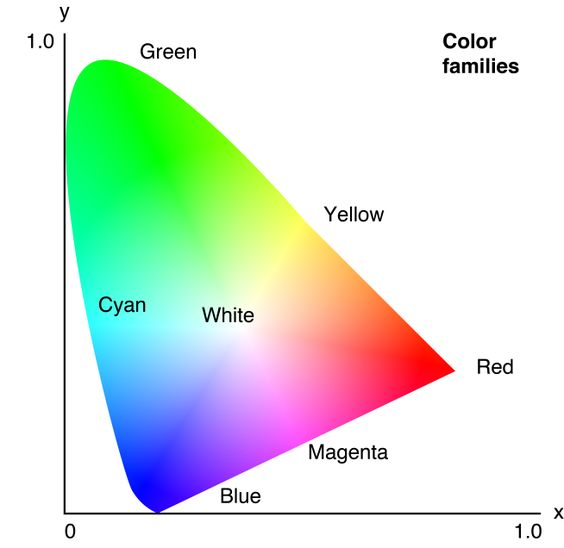
\includegraphics[scale=0.5]{cieYxy}
\newpage
\item \textbf{RGB}: una vasta percentuale dello spettro visibile può essere rappresentata miscelando i 3 componenti della luce colorate Rosso, Verde e Blu in diverse proporzioni e intensità.\\
Vengono chiamati colori addittivi perchè se sommiamo questi 3 colori generiamo il colore bianco. I colori addittivi vengono usati per l'illuminazione, i video e i monitor.\\

\includegraphics[scale=0.5]{rgb}
\newpage
\item \textbf{CMYK}: questo modello si basa sulla capacità di assorbimento della luce dell'inchiostro sulla carta. Quando la luce bianca colpisce gli inchiostri traslucidi, una parte dello spettro viene assorbita e una parte viene riflessa all'occhio.\\ 
I pigmenti puri di Cyan, Magenta e Giallo si sommano per assorbire tutto il colore e produrre il Nero: per questo sono chiamati colori sottrattivi.\\ 
La combinazione di questi inchiostri per riprodurre il colore viene chiamata stampa in quadricomia.\\

\includegraphics[scale=0.5]{cmyk}
\end{enumerate}
\subsubsection{Spazio colore}
Lo spazio colore indica l'intervallo dei colori che possono essere visualizzati o stampati.\\
Lo spettro dei colori percepiti dall'occhio umano è maggiore di qualsiasi metodo di riproduzione del colore.\\
Fra i vari modelli del colore, CIE ha lo spazio colore più ampio, e comprende gli spazi di colore di RGB E CMYK.\\
Ci sono diversi spazi colore RGB: ad esempio, sRGB (disegnato in relazione alle possibilità di visualizzazione dei monitor CRT, gamma molto ristretta), Adobe RGB (che include la maggior parte dei colori ottenibili sulle stampanti CMYK ma utilizzando colori primari RGB, gamma molto più ampia di sRGB), Adobe WWide Gamut RGB (versione estesa di Adobe RGB).\\
È necessario tenere in considerazione che questi sono modelli teorici rispetto ai quali i singoli dispositivi riescono ad adeguarsi in modo diverso.
\subsubsection{Pixel}
Per controllare il colore di ogni pixel sullo schermo il sistema operativo deve dedicare una piccola quantità di memoria ad ognuno di essi.\\
La memoria dedicata allo schermo è una memoria distinta, che risiede nella scheda grafica e ci si riferisce con Video RAM (VRAM).\\
\subsubsection{Colore RGB digitale}
Per ogni pixel, abbiamo:
\begin{itemize}
\item HIGH COLOR: 16 bit, 5 bit per componente (il sedicesimo bit utilizzato per altri scopi).
\item TRUE COLOR: 24 bit, 8 bit per ogni componente. Se si utilizzano 32 bit per pixel, i bit aggiuntivi vengono riservati per velocizzare le operazioni della scheda grafica o per informazioni di mascheratura/trasparenza.
\item DEEP COLOR: 16/32/48/64 bit per componente.
\end{itemize}
\paragraph{Colore RGB a 24 bit\\}
Con schede grafiche RGB a 24 bit, viene assegnato un valore di intensità a ogni pixel compreso tra 0 (nero) a 255 (bianco) per ognuna delle componenti RGB di un'immagine a colori.
Le immagini RGB utilizzano 3 colori per riprodurre fino a 16,7 milioni di colori sullo shcermo.
\subsubsection{Discretizzare il reale}
La realtà percepita dall'occhio umano è a tono continuo. Catturare un'immagine con strumenti digitali vuol dire discrettizare l'informazione contenuta nella scena reale.
\subsubsection{Colori per il Web}
Per specificare i colori RGB è quello di utilizzare il valore numerico della tripletta di componenti, convertiti in notazione esadecimale.\\
Su sistema hardware dotati capacità grafiche inferiori (8-16 bit) i colori provenienti da uno spazio colore true space (ossia a 24 bit) vengono approssimati. \\
Per operazioni a livello di sistema i computer utilizzano un set specifico di 256 colori, chiamato palette di sistema.\\
Ogni sistema operativo ha la sua palette. Per questo motivo è stata introdotta una web-safe palette, che consiste di 216 colori comuni alle palette di sistema Win e Mac.\\
Tutti i colori della web palette sono combinazioni dei valori esadecimali 00,33,66,99,CC,FF.\\
L'utilizzo di colori che non appartengono alla web palette su computer con scarse risorse grafiche può portare ad una approssimazione del colore (dithering) e a risultati sgradevoli.\\
\subsubsection{Gamma}
La gamma denota la luminosità complessiva del display. Più è alto il valore, meno luminosa è l'immagine sul display. Notare che ogni piattaforma ha una gamma diversa, quindi immagini create su Mac appaiono più scure sui sistemi Win.
\subsection{Progettare il layout}
Nel design tradizionale, le dimensioni del supporto vengono stabilite a priori e costituiscono un vincolo immutabile durante la progettazione del layout.\\
Nel design tradizionale viene definita la gabbia tipografica, che partiziona lo spazio disponibile in aree omogenee le quali conterranno testo, grafica, o (nel caso di supporti elettronici) elementi multimediali. È un elemento caratterizzante del design complessivo, quindi da mantenere costante durante la pubblicazione.
\subsubsection{Prodotto editoriale stampato}
Nei giornali è presente un modulo verticale (principalmente su 8 colonne) che costiuisce la base del layout del quotidiano.\\
Tutti gli altri elementi sono costruiti basandosi su questo modulo di base, rispettando allineamenti e regole di simmetria.\\
Per convenzione, la pubblicità viene posizionata nei due riquadri superiori e nella base del layout. L'articolo di fondo è sempre posizionato a sinistra. La zona superiore viene riservata alle notizie generali rilevanti mentre quella inferiore alla cronaca locale.
\subsubsection{Vantaggi della gabbia tipografica}
\begin{itemize}
\item Aspetti funzionali: magiore facilità nel reperimento dell'informazione da parte del lettore e maggiore facilità nell'interazione con i prodotti editoriali interattivi da parte dell'utente.
\item Aspetti comunicativi: è l'elemento fondamentale dell'identità di un progetto grafico.
\item Creatività: è possibile coniugare rigore e creatività, introducendo eccezioni rispetto alla regola data.
\end{itemize}
\subsubsection{Progettare layout web}
\begin{itemize}
\item Supporto: problematico assicurare la corrispondenza tra la dimensione complessiva della pagina e l'area visibile all'utente.
\item Controllo del layout: nelle prime versioni di HTML non era possibile alcuna forma di controllo del layout della pagina. Il CSS permette un controllo accurato del layout, permettendo anche di ottenere layout diversi per media diversi.
\end{itemize}
\subsubsection{Area sicura}
\begin{itemize}
\item Per la visualizzazione: numero di punti dello schermo (pixel) disponibili per visualizzare l'informazione di una pagina web.
\item Per la stampa: numero di punti dello schermo stampabile su carta.
\end{itemize}
L'area sicura dipende da configurazione HW e SW, browser e preferenze dell'utente.
Nell'area sicura è meglio mettere gli elementi informativi fondamentali, gli artefatti fondamentali per l'interazione con il sito, e gli elementi grafici caratterizzanti.
\subsubsection{Layout flessibili e fissi}
\begin{itemize}
\item Layout flessibile: dimensioni delle aree fissate usando misure relative (es percentuale) come anche le dimensioni del carattere, per permetterne uno zoom e un rimpicciolimento. \\
Vantaggi: pagina si adatta al display e alle preferenze dell'utente.\\
Svantaggi: in alcuni casi possono verificarsi righe troppo lunghe e non facilmente leggibili.
\item Layout fissi: dimensioni fissate usando misure assolute (es pixel).\\
Vantaggi: risultato unico, maggior controllo.\\
Svantaggi: problemi su determinate configurazioni HW  e SW (ad esempio IE fino alla versione 6 non permette all'utente di riscalare un testo le cui dimensioni siano state fissate in pixel. Non viene garantito il controllo sul carattere tipografico (come descritto nella sezione font).
\end{itemize}
La scelta della tipologia di layout dipende da diversi fattori, ad esempio gli utenti, l'ambiente e la tipologia di servizio offerto.\\
È preferibile l'adozione di layout flessibili, che permettono un migliore adattamento a dispositivi eterogenei.
\section{Pianificare un sito web}
Progettare e sviluppare siti web è un'attività complessa che richiede un team di sviluppo interdisciplinare.
\begin{itemize}
\item Project Manager: responsabile coordinamento team, si occupa della schedulazione dei task e del controllo del budget.
\item Esperto in marketing: identifica obiettivi del sito e utenti.
\item Information Designer: è il responsabile dei sistema di strutturazione, classificazione, ricerca e navigazione all'interno del sito.
\item Informatico: amministra il server, sviluppa e tiene aggiornati servizi e app.
\item Web Designer: progettista del design e del layout. Crea relazioni tra gli elementi del sito.
\item Giornalista/Responsabile editoriale: prepara e adatta i testi da inserire nel sito.
\item Esperto in usabilità: responsabile valutazione usabilità dei prototipi e del sito finale.
\end{itemize}
\section{Architettura dell'informazione}
Cos'è l'architettura dell'informazione?
\begin{itemize}
\item il design strutturale di ambienti informativi condivisi
\item la combinazione di organizzazione, etichettatura, ricerca e sistemi di navigazione relativi a siti web e intranet
\item l'arte e la scienza di dare forma a prodotti ed esperienze informative per supportare l'usabilità e la trovabilità.
\end{itemize}
Nell'archittettura dell'informazione troviamo Sistemi (sistemi di ricerca, di navigazione, reti semantiche) e prodotti (strutture organizzative, vocabolari controllati, metadati, layout).
\subsection{I 3 cerchi dell'architettura dell'informazione}
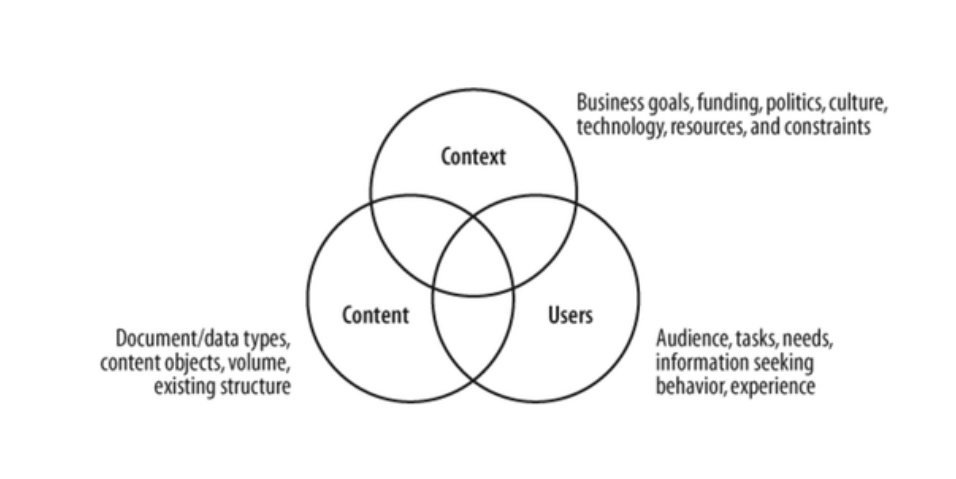
\includegraphics[scale=0.5]{3cerchi}
\begin{itemize}
\item Contenuti: includono documenti, applicazioni, servizi, schemi e metadati. I parametri da considerare includono il produttore e il proprietario dei contenuti, il formato, la granularità, i metadati, il volume e la dinamicità dei contenuti.
\item Contesto: i siti vengono definiti all'interno di un determinato contesto, con una missione specifica, obiettivi, strategia, staff, processi e procedure. L'architettura dell'informazione di un sito deve fornire un'immagine tangibile dell'organizzazione che lo promuove.
\item Utenti: esistono diversità nelle preferenze degli utenti e nei comportamenti.
\end{itemize}
Contenuto, utenti e contesto sono componenti interdipendenti nell'ambito del processo di definizione dell'informazione.
\subsection{Bisogni e comportamenti degli utenti}
\paragraph{Modello informativo too-simple}
\begin{itemize}
\item utente pone una domanda
\item accade qualcosa
\item utente riceve risposta
\item fine ricerca
\end{itemize}
I problemi che possono sorgere sono che l'utente non sempre sa quello che vuole. Inoltre spesso la ricerca termina con un insuccesso, o un successo parziale. Il contesto viene ignorato.
\subsubsection{Che cosa vogliono gli utenti?}
Ci sono diversi tipi di bisogno, possiamo definirli con la metafora della pesca:
\begin{itemize}
\item \textbf{Il tiro perfetto}: quando gli utenti sanno quello che stanno cercando.
\item \textbf{Trappola per aragoste}: gli utenti non hanno un'idea precisa di quello che stanno cercando, si aspettano di trovare qualcosa e di imparare qualcosa dal processo espolorativo, che possa guidarli verso una nuova ricerca.
\item \textbf{Pesca con la rete}: utenti vogliono esaminare ogni elemento relativo ad un particolare argomento
\item \textbf{Boa di segnalazione}: gli utenti vogliono ritrovare un elemento informativo utile
\end{itemize}
\subsubsection{Comportamenti dell'utente}
Gli utenti trovano l'informazione mediante:
\begin{enumerate}
\item searching (ricerca)
\item browsing (navigazione)
\item asking (facendo domande)
\end{enumerate}
Searching, browsing e asking spesso sono integrati nella stessa sessione di lavoro, oppure utilizzati in iterazione.
\subsubsection{Modello berry-picking}
Gli utenti partono con un bisogno informativo, formulano una query (rihiesta informativa), e si muovono iterativamente attraverso percorsi potenzialmente complessi, raccogliendo progressivamente elementi informativi. Se il comportamento degli utenti rispecchia questo modello, è necessario che sia possibile spostarsi facilmente tra searching e browsing.
\subsubsection{Modello pear-growing}
Gli utenti partono con uno o pochi documenti che corrispondono esattamente a quello di cui hanno bisogno per cercare altri documenti con quelle caratteristiche (es. pagine simili di Google, oppure ritrovare documenti indicizzati con le stesse keyword).
\subsection{Progettare la struttura dell'informazione}
Internet dà la libertà di pubblicare l'organizzazione e la responsabilità di organizzarla (nel passato quest'ultimo compito era svolto da figure professionali come i bibliotecari).
\subsubsection{Problemi nell'organizzazione dellinformazione}
\begin{itemize}
	\item Ambiguità: i sistemi di classificazione sono basati su un linguaggi (che può essere ambiguo), inoltre classificare oggetti e concetti astratti può essere difficoltoso.
	\item Eterogeneità: molti siti web sono eterogenei, forniscono cioè l'accesso a documenti a diversi livelli di granularità e formati multipli.
	\item Differenze di prospettiva: è indispendabile mettersi nei panni dell'utente.
	\item Diversità di politiche
\end{itemize}
\subsection{Organizzare l'informazione}
\subsubsection{Schemi organizzativi}
Permettono di suddividere gli oggettii informativi in raggruppamenti logici basandosi su proprietà caratterizzanti dei singoli oggetti. Sono suddivisi in schemi organizzativi esatti e ambigui.
\begin{itemize}
	\item \textbf{Esatti}: l'informazione viene suddivisa in sezioni mutuamente esclusive. La progettazione e la manutenzione è facile, ma richiedono che l'utente conosca il nome specifico della risorsa che sta cercando (know-item searching). Degli esempi sono: schema alfabetico, schema cronologico, schema geografico. 
	\item \textbf{Ambigui}: sono utili per realizzare e soddisfare uno stile di ricerca basato sulla serendipità. L'informazione è suddivisa in categorie nelle quali può essere difficile collocare l'oggetto. Sono più importanti e utili dei schemi organizzativi esatti, nel caso in cui non sappiamo che cosa stiamo cercando (exploratory searching).\\
	In questo caso la serendipità può essere supportata implementando una ricerca iterativa e interattiva, e coinvolgendo meccanismi di apprendimento associativo.\\
	Gli schemi organizzativi ambigui più comuni sono: schemi per argomento (topical, andando a definire l'universo degli argomenti che l'utente si aspetta di trovare), schemi orientati al compito (task oriented, dove il contenuto e le applicazioni sono organizzati come collezioni di processi, funzioni o compiti), schemi specifici per audience, schemi metaforici (utilizzati per far comprendere concetti nuovi collegandoli a concetti familiari, da usare con cautela ed è necessario evitare problemi di inconsistenza), schemi ibridi (mix di tutto).
\end{itemize}
Le facets (sfaccettature) permettono di accedere allo stesso informativo da angolature (schemi organizzativi) diversi. Definire più facets permette all'utente una maggiore interazione in quanto può navigare in diversi modi, è possibile inoltre associare una caratteristica dell'oggetto al facets (ad esempio un negozio di vestiti può essere navigato per marca, colore, taglia, ...).
\subsubsection{Strutture organizzative}
Definiscono le tipologie di relazione tra elementi o gruppi di oggetti dell'universo informativo. Esistono diverse strutture organizzative, ognuna con i sui punti di forza e debolezze.
\begin{itemize}
	\item \textbf{Sequenze}: l'informazione è messa in sequenza. Le sequenze lineari sono adatte a siti didattici in cui l'utente deve procedere ordinatamente attraverso un insieme di materiali.
	\item \textbf{Gerarchia}: c'è un livello di parentela tra le informazioni, come una struttura ad albero. Gli utenti che utilizzano questa organizzazione sono in grado di sviluppare più facilmente un modello mentale della struttura del sito.\\
	Le categorie gerarchiche dovrebbero essere mutuamente esclusivo ma non è illegale posizionare un numero limitato di oggetti informativi in più di una categoria (cross listing) per creare una struttura poligerarchica. Posizionare un numero eccessivo di elementi in più cateagoria porta una perdita di valore di questa struttura.\\
	È necessario inoltre definire un equilibrio tra ampiezza (numero di opzioni ad ogni livello) e profondità (numero di livelli) della gerarchia (non oltre 10 opzioni, e 4 o 5 livelli).
	\item \textbf{Ipertesto}: innotiva modalità non lineare per strutturare l'informazione.\\
	Le unità informative possono essere collegate gerarchicamente, non gerarchicamente o in entrambe le modalità.\\ Può essere un ostacolo per la formazione di un modello mentale del sito 
	\item \textbf{Database}: è una collezione di record, dove ogni record ha un numero n di campi associati. I vantaggi sono: ricerca per campo, metadati associati ai dati, vocabolario controllato (imponibile un grado di consistenza che può risultare utile nella ricerca e navigazione), gestione più facile dei contenuti. Gli svantaggi sono che la strutturazione a record è rigida, e può essere costoso disporre ogni elemento del sito in un database.\\
	È utile usare un database per rappresentare una collezione di oggetti con le stesse proprietà. Molto spesso un datbase viene usato per modellare anche gli altri elementi strutturali del sito e non solo il contenuto principale.
\end{itemize}
\subsubsection{Approccio top-down}
Le strutture organizzative viste precedentemente vengono costruito usando un approccio top-down: l'information designer fornisce una soluzione relativa ad un dominio informativo per un determinato sito web.\\
Spesso, però, non tutti gli utenti trovano una corrispondenza tra la struttura progettata dal designer e il proprio modello mentale relativo al sito. Per limitare questi problemi è possibile fornire soluzioni poligerarchiche, motori di ricerca interni, mappe del sito oppure permettere agli utenti di costruire la gerarchia informativa con tecniche quali il free listing e il card sorting.
\begin{itemize}
	\item \textbf{Free listing}: permette di coinvolgere gli utenti nella definizione dei contenuti del dominio. Viene richiesto di formulare un elenco di elementi informativi a partire dalla descrizione di un tema fornita da chi gestisce il test.
	\item \textbf{Card sorting}: permette di coinvolgere gli utenti nella strutturazione dei contenuti. Viene richiesto di sudividere in gruppi una lista di schede etichettate. Si può usare l'open card sorting (agli utenti vengono fornite schede con etichette relative al contenuto del sito ma senza gruppi prestabiliti; l'utente deve quindi creare i gruppi e assegnare le etichette descrittive dei gruppi stessi), o il closed card sorting (agli utenti vengono fornite sia le schede con etichette dei contenuti del sito, sia i gruppi con le etichette già definite; l'utente deve riempire i gruppi con le schede). L'open card viene usato per creare un'architettura informativa, per ottenere feedback su quali contenuti vengono inseriti in uno stesso gruppo, e capire quali etichette vengono utilizzate dagli utenti per descrivere il contenuto.
	Il closed card sorting, invece, risulta utile per testare il design di un'architettura dell'informazione, e per ricevere feedback sull'efficacia delle etichette.
\end{itemize}
Il free listing e il card sorting mirano ad aumentare la trovabilità degli elementi di un sito web.
Per validare la gerarchia di un sito viene usato il tree testing: all'utente viene proposto una serie di task consistenti nel trovare un determinato elemento informativo facente parte di una struttura gerarchica. L'utente una volta raggiunto l'elemento informativo che reputa corretto deve confermare la scelta. In un tree testing vengono considerati: tempo impiegato, precisione (percentuale di utenti che non sono tornati indietro) e percentuale di successo.
\subsubsection{Approccio botttom-up}
Si costruisce la struttura informativa dal basso, dando modo all'utente di marcare gli elementi informativi che sta navigando con un set di tag. Una tecnica è il free tagging, ossia categorizzazione collaborativa di elementi informativi del web che può far emergere una forma di organizzazione complementare (o alternativa) all'approccio top-down.\\
Si può usare una folksnonomia allargata (accettati tutti i possibili tag, anche ripetuti, usata da Delicious) o una folksonomia ristretta (per ogni risorsa il sistema non accetta che un utente inserisca tag già inseriti da altri utenti, usata da Flickr).
I vantaggi di questo approccio sono: l'approccio è meglio di niente, in quanto molte volte non è sempre possibile trovare e applicare un vocabolario controllato a tutte le situazioni.
Gli svantaggi invece sono: non c'è una maggiore trovabilità degli elementi, molto spesso viene ignorata l'importanza del contesto, e la mancanza di un vocabolario controllato può creare diversi problemi legati alla semantica, all'ononimia (stesso tag per concetti diversi), polisemia, desinenze. Per risolvere alcuni limiti è possibile suggerire all'utente i tag da inserire da una lista di popular tag o da una lista di tag raccomandati, oppure visualizzando una lista di termini le cui lettere iniziali corrispondono ai caratteri inseriti dagli utenti.
\subsubsection{Creare sistemi organizzativi coesi}
Usare schemi organizzativi esatti se l'utente sa quello che sta cercando, altrimenti utilizzare schemi ambigui, che sono migliori per la navigazione e l'apprendimento associativo. Quando è possibile è opportuno utilizzare entrambi i tipi di schema.
\section{Sistemi di navigazione}
I sistemi di navigazione devono fornire all'utente il contesto, devono permettere all'utente di spostarsi in modo flessibile tra le unità informative. È necessario bilanciare la flessibilità e la fornitura di troppe opzioni.
\subsection{Il design di sistemi di navigazione}
L'utente si sposta attraverso le unità informative di un sito web in due modi:
\begin{itemize}
	\item Browsing (selezione di elementi ipertestuali presenti nella presentazione di partenza, organizzati in gruppi e facenti riferimento alle strutture organizzative del sito)
	\item Searching (navigazione attraverso un'interrogazione del sistema, svolta attraverso la compilazione di un modulo e la selezione di una della unità informative proposte come risposta)
\end{itemize}
Integrare questi due meccanismi permette ad un utente di navigare nel sisto attraverso una modalità mista.\\
Molti browser inoltre forniscono un supporto alla navigazione (aprire un url per accesso diretto, bookmarks, uso di colore nei link ipertestuali, tasti avanti e indietro). Non bisogna danneggiare questo sistema di navigazione (modificare colore link, rimuovere sottolineatura dei link, nascondere l'url di destinazione)
\subsection{Costruire il contesto}
È necessario costruire quindi un contesto, ad esempio includendo in tutte le pagine il nome dell'ente/azienda oppure un logo e presentando in tutte le pagine la struttura dell'informazione gerarchica e la posizione dell'utente rispetto ad essa.
\subsection{Navigation Stress Test}
È utile per verificare la capacità di un sito di rappresentare il contesto.
Si parte da una pagina a caso, e si rispondono alle domande:
\begin{itemize}
	\item So dove sono?
	\item In che sezione principale del sito mi trovo?
	\item Qual'è la pagina padre di questa pagina?
	\item Dove mi condurrà la pagina in cui mi trovo?
	\item I link suggeriscono la destinazione?
	\item I link sono abbastanza differenziati per aiutarmi a scegliere un link piuttosto che un altro?
\end{itemize}
\subsection{Tipologie di Sistemi di Browsing}
Un sito complesso può includere diversi sistemi di navigazione.
\subsubsection{Sistema Gerarchico}
Gerarchia informativa, permette la navigazione da elementi padre ad elementi figlio, e viceversa.
\subsubsection{Sistema Globale}
Permette la navigazione verticale (da elementi padre a figlio, anche a passi maggiori di 1) e la navigazione orizzontale (tra elementi dello stesso padre).
\subsubsection{Sistemi Locali}
Sistema di navigazione utilizzato in un sottosito, cioè in una sezione del sito nella quale le unità informative sono legate da relazioni peculiari (es. catalogo online di un'azienda). È importante estendere il sistema Globale anche all'interno di sottositi.
\subsubsection{Sistemi Ad hoc - Trasversali - Contestuali}
Le relazioni tra contenuti informativi non riconducibili ad attraversamenti verticali o orizzontali della gerarchia, ad esempio i links contenuti nel corpo di un paragrafo (embedded links) oppure links evidenziati separatamente del layout della pagina.
\subsection{Elementi di browsing integrati}
\subsubsection{Menu di navigazione}
È una collezione di links ipertestuali, sottoforma di testo, imagemap o immagini separate.\\
La progettazione dell'architettura può influenzare la scelta dell'implementazione. Ad esempio, siti con aree in espansione o variabili scelgono soluzioni testuali. Per la navigazione globale è opportuno usare una barra grafica, per la navigazione locale una barra testuale.\\
I menu permettono di effettuare la navigazione orizzontale all'interno del sito.\\
\subsubsection{Shortcuts}
Sono elementi di navigazione che risiedono tipicamente nella home page di un sito: possono essere singoli oppure utilizzati in gruppi.\\
Permettono all'utente un accesso diretto a elementi che si trovano nei livelli più profondi della gerarchia informativa del sito (sono una navigazione verticale).\\
Sono associati all'esigenza di rendere noto all'utente l'esistenza di un elemento o di un gruppo di elementi informativi.
\subsubsection{Menu pop-up e pull-down}
Permettono di rappresentare molti link in forma compatta, nascondono opzioni. Vegono utilizzati per effettuare selezioni secondarie oppure in contesti informativi molto affollati. È sconsigliato utilizzarli per le opzioni informative principali nei sistemi desktop (nei layout per smartphone invece è possibile utilizzarli per ottimizzare lo spazio).\\
È opportuno che la riga di menù visibile indichi la tipologia dell'informazione.\\
È possibile anche specificare eventi che possono attivare l'apertura del menu (ad esempio uno swipe, la pressione di un tasto, al passaggio del mouse).
\subsubsection{Drawer}
I drawer permettono di rappresentare links in forma compatta: può essere utile utilizzarli nei casi in cui sia necessario un livello di strutturazione elevato dei menu pop-up e pull-down.\\
Vengono utilizzati nei dispositivi con uno schermo piccolo.
\subsection{Sistemi di browsing}
\begin{itemize}
	\item Navigazione gerarchica (può essere molto limitante)
	\item Navigazione globale
	\item Navigazione locale
	\item Navigazione trasversale
	\subitem Embedded links (navigazione adhoc con link nel testo)
	\subitem Navigazione trasversale
	\subitem See also
\end{itemize}
\subsection{Elementi di browsing remoti}
Sono elementi che forniscono un punto di vista esterno alla gerarchia base del sito.
Sono utilizzati come complemento agli elementi di navigazione integrati.\\
\subsubsection{Indice dei contenuti}
Rappresenta i livelli della gerarchia informativa, l'indice attivo (che impiega link ipertestuali) facilità l'accesso non lineare ai contenuti.\\
È utile utilizzarlo quando il sito ha un'organizzazione gerarchica.
\subsubsection{Indice analitico}
Alternativa per siti che non hanno ua forte organizzazione gerarchica.\\
È utile per gli utenti che sanno quello che stanno cercando; gli elementi dell'indice devono puntare a componenti del sito dove prevalgono i contenuti piuttosto che a componenti dove prevalgono le strutture di navigazione.
\subsubsection{Mappa del sito}
È una rappresentazione grafica dell'architettura di un sito.\\
La mappa evidenzia le relazioni tra le componenti informative.\\
Deve rappresentare gli elementi informativi importanti e le loro relazioni in modo chiaro e significativo.\\
Le mappe non si prestano ad una lettura TTSS, è preferibile quindi affiancare una mappa ad un indice dei contenuti.
\subsubsection{Tour guidato}
Utile per introdurre ai nuovi utenti i contenuti del sito. Dovrebbe avere una navigazione lineare ed essere eseguibile dalla home page del sito.
\subsection{Sistemi di browsing personalizzati}
Possiamo distinguerli in:
\begin{itemize}
\item Adattivi: le opportunità di navigazione vengono selezionati dal sistema in abse ad alcuni parametri, come il profilo dell'utente o lo storico di utilizzo.
\item Adattabili: l'utente può scegliere diverse opzioni di navigazioni differenziate.
\end{itemize}
\subsection{Sistemi di navigazione sociale}
Permettono all'utente di navigare il sito utilizzando l'attività di tagging degli altri utenti, si costruisce quindi una folksnomia in modo progressivo.\\
Può essere l'unico sistema di navigazione oppure affiancarne un altro.
\subsubsection{Tag clouds}
Una folksonomia è rappresentata da una tagcloud, che esprime la frequenza di utilizzo dei tag attraverso la dimnesione del carattere tipografico. Può essere costruita a partire da una folksonomia allargata che ristretta. 
\subsubsection{Interfaccia per l'inserimento di tag}
Oltre all'interfaccia di navigazione può essere presente l'interfaccia di inserimento dei tags (nei sistemi di tipo bottom-up l'utente può contribuire ad arricchire la classificazione).
\subsubsection{Integrazione nel layout delle interfacce di navigazione sociale}
Le interfacce dei sistemi di navigazione possono essere presenti nel layout del sito specifico, nel layout di un altro sito che funge da collettore di tagging degli utenti sul web, oppure secondo modalità miste.
\subsubsection{Utenti, risorse e annotazioni}
\begin{enumerate}
	\item Annotazioni top-down: i singoli siti forniscono all'utente fornitore di contenuti le interfacce per inserire risorse e annotarle. L'utente che gestisce la singola risorsa coincide con l'utente autorizzato ad annotare la risorsa (solo lui può annotare la risorsa). Abbiamo una integrazione totale dell'interfaccia di annotazione nel layout.
	\item Annotazioni bottom-up tipo 1: le risorse informative e le annotazioni risiedono in unico repository. Le interfacce e le risorse per annotarle sono fornite da un gestore unico.\\
	Abbiamo comunque un'integrazione totale delle interfacce di annotazione nel layout di presentazione, ma in questo caso è consentito ad utenti diversi l'annotazione di risorse gestite da altri.
	\item Annotazioni bottom-up tipo 2: le risorse informative e le annotazione risiedono in siti diversi. È difficile quindi un'integrazione delle interfacce di annotazione nel layout di presentazione delle risorse informative.
\end{enumerate}
\subsubsection{Fake tagcloud}
Esistono anche della tagcloud fake: in questo caso i contenuti della tagcloud, e la grandezza delle parole è una scelta redazionale, per mettere in risalto alcuni contenuti. In questo caso, non possiamo parlare di tagging sociale.
\section{Sistemi di ricerca}
\subsection{Quando implementare un sistema di ricerca?}
\begin{itemize}
	\item Quando abbiamo molta informazione da percorrere attraverso sistemi di browsing
	\item Quando il sito è costituito da componenti frammentati
	\item Quando dobbiamo imparare dagli utenti (analisi search-logs)
	\item Quando gli utenti si aspettano che ci sia
	\item Quando il sito è dinamico
\end{itemize}
\subsection{Zone di ricerca}
Non è sempre opportuno indicizzare tutto il sito.\\
Creare search-zones riduce l'effetto apple-and-oranges, ossia la ricerca effettuata su aree eterogenee di contenuti che può essere un ostacolo al ritrovamento dell'informazione.\\
Le zone di ricerca sono parti di sito che sono state indicizzate separatamente.\\
Si possono creare suddividendo logicamente o fisicamente i documenti. È possibile crearla a partire da schemi e strutture organizzative.\\
Con le zone di ricerca però andiamo ad aggiungere un ulteriore complessità alla ricerca.
\subsection{Pagine di destinazione e navigazione}
Le pagine di destinazione contengono il contenuto vero e proprio.\\
Le pagine di navigazione hanno lo scopo di condurre gli utenti verso le pagine di destinazione. Non vengono indicizzate.\\
Spesso, le pagine appartengono ad entrambe le categorie.
\subsection{Componenti di una pagina}
La nascita dei sistemi CMS (Content Management System) rende più facile l'identificazione degi elementi della pagina (contenuto informativo, menu di navigazione, pubblicità, disclaimers...) e la loro inclusione o meno dall'indicizzazione. Usare un CMS permette di selezionare gli elementi da indicizzare ad un livello di granularità più accurato rispetto a quello della pagina.
\subsection{Presentare i risultati}
\subsubsection{Quali?}
\begin{itemize}
	\item mostrare come risultato all'utente che sa quello che sta cercando meno informazione rispetto a quella presentata all'utente che non sa quello che sta cercando.
	\item Agli utenti del primo caso possono bastare alcuni elementi rappresentativi del contenuto.
	\item La seconda categoria di utenti richiede contenuti più descrittivi.
	\item In alcuni casi, l'utente può scegliere cosa visualizzare.
\end{itemize}
\subsubsection{Quanti?}
Dipende da due fattori, dalla quantità di componenti informativi per componente e dalla caratteristica del dispositivo.\\
Si parte dalla presentazione di un gruppo limitato di documenti (10 per pagina) e si lascia la laibertà di configurare al sistema.\\
È opportuno visualizzare il numero complessivo di documenti ritrovati e fornire un sistema di browsing per permettere una rapida navigazione tra i risultati.
\subsubsection{Elencare i risultati}
Esistono due metodi per elencare i risultati.\\
Sorting: i risultati vengono ordinati secondo un criterio basato su una della componenti del documenti (utile quando l'utente deve comparare due o più documenti).\\
Ranking: risultati ordinati con criteri come la rilevanza del documento, dedotta analizzandone i contenuti (condiderando quanti termini della query sono presenti nel documento e quante volte, la vicinanza e la locazione di questi termini)o la sua popolarità. (ad esempio PageRank di Google). Oppure può essere realizzato un ranking attraverso il giudizio di esperti, i quali valutano il valore dell'informazione, o attraverso un modello pay-for-placement.
\subsubsection{Ragruppare i risultati}
Una tecnica alternativa (o complementare) al Sorting e al Ranking consiste nel raggruppare i risultati in base a qualche aspetto comune.\\
Come possiamo raggruppare i risultati? Attraverso l'utilizzo di metadati (tipo di documento, data creazione), attraverso l'uso di metadati applicati manualmente (audience, contenuto, tags). Alcuni tool cercano di derivare autonomamente alcuni cluster di contenuti considerando i contesti possibili a partire da una keyword inserita dall'utente.
\subsubsection{Esportare i risultati}
Un utile complemento può essere quello di esportare i risultati (stampare, inviare via mail, salvare).\\
Quando si vuole salvare un insieme di elementi interessanti è utile fornire una selezione di un sottoinsieme di risultati.\\
Il salvataggio di una ricerca, inoltre, è un'alternativa utile per i domini dinamici, per i quali la riesecuzione dell'interrogazione in un altro momento può portare nuovi risultati.
\subsection{L'interfaccia di ricerca}
È necessario mantenere l'interfaccia di ricerca il più semplice possibile. L'utente non deve utilizzare operatori logici, non deve preoccuparsi di utilizzare un vocabolario controllato e la ricerca viene fatta sull'intero sito.\\
Per educare l'utente è possibile creare una pagina di consigli, oppure inserire la possibilità di restringere la ricerca ad una search zone o inserendo un collegamento ad un modulo di ricerca avanzata.
\subsection{L'interfaccia per i risultati}
È necessario fornire un supporto alla revisione, ad esempio descrivendo gli eventuali filtri applicati, mostrando gli operatori booleani applicati implicitamente alla ricerca, mostrando le caratteristiche utilizzate per la presentazione (ad esempio il tipo di sorting) ed evidenziando il numero dei risultati ottenuti dalla ricerca.
\subsection{Interfacce di ricerca basate sulla classificazione sociale}
In alcune situazione sono disponibili sistemi di ricerca dei tags.\\
Succede per le situazioni in cui i tags costituiscono il sistema prevalente di classificazione dell'informazione o nei sistemi caratterizzati dalla presenza di molti tags associati alle risorse.\\
È importante rendere consapevole l'utenza che la ricerca delle informazioni avviene sull'insieme dei tags e non sull'insieme delle parole che compongono la pagina web.\\
\subsection{Trovabilità}
La trovabilità è definita come $ Finding = Searching + Browsing$. Per aumentare la trovabilità degli elementi è necessario quindi integrare le due modalità di navigazione di un sito, rendendo possibile passare da una navigazione ad un'altra in modo semplice.
\end{document}